\addsection{Resources}{\images/estates.png}
\hypertarget{Resources}{There} are three types of resources in the game: Gold \includesvg[height=10px]{\svgs/gold.svg}, Building materials \includesvg[height=10px]{\svgs/BuildMat.svg}, and Valuables \includesvg[height=10px]{\svgs/valuablegreater.svg}.
Resources are spent during the game to expand your \hyperlink{Town}{Town}, to recruit \hyperlink{Units}{Units}, and to purchase \hyperlink{spells}{Spells}.
You can gain Resources from the \hyperlink{Mines}{Settlements and Mines} that you have \hyperlink{Categories}{Flagged}, but also by playing cards and rolling Resource Dice \includesvg[height=10px]{\svgs/resource_die.svg}.
Whenever a player's resource production is increased or decreased, move that Resource's cube on its production track the appropriate number of spaces.\par
\begin{figure}[h]
  \centering
  \minipage[b]{0.32\textwidth}
    \centering
    
\includegraphics[scale=0.2]{\images/gold.png}
    \caption{{\textit{\textbf{\textcolor{darkcandyapplered}{Gold}}}}}
  \endminipage
  \minipage[b]{0.32\textwidth}
    \centering
    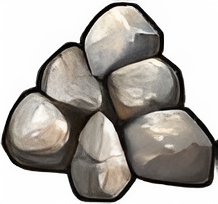
\includegraphics[scale=0.2]{\images/building_materials.png}
    \caption{{\textit{\textbf{{\textcolor{darkcandyapplered}{Building Materials}}}}}}
  \endminipage
  \minipage[b]{0.32\textwidth}
    \centering
    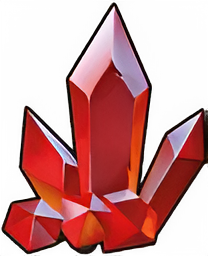
\includegraphics[scale=0.2]{\images/valuables.png}
    \caption{{\textit{\textbf{{\textcolor{darkcandyapplered}{Valuables}}}}}}
  \endminipage
\end{figure}
Players start each scenario with the number of resources indicated in that scenario’s set up.
Resources can also be \hyperlink{Trading}{traded}.
There's no limit to the amount of resources you can have.\bigbreak

\begin{minipage}[T]{0.38\textwidth}
    Possible Resource Die \includesvg[height=10px]{\svgs/resource_die.svg} results:\bigbreak
    \begin{itemize}
        \setlength\itemsep{10pt}
        \item \includesvg[height=15px]{\svgs/2BuildMat.svg} - 2 x Building Materials
        \item \includesvg[height=15px]{\svgs/4BuildMat.svg} - 4 x Building Materials
        \item \includesvg[height=15px]{\svgs/1valuables.svg} - 1 x Valuables
        \item \includesvg[height=15px]{\svgs/2valuables.svg} - 2 x Valuables
        \item \includesvg[height=15px]{\svgs/3gold.svg} 3 x Gold
        \item \includesvg[height=15px]{\svgs/6gold.svg} 6 x Gold
    \end{itemize}
\end{minipage}
\begin{minipage}[t]{0.48\textwidth}
    \shadowimage[width=0.88\textwidth]{\images/resource_board.png}
    \break
    \centering
    \footnotesize{\textbf{\textit{\textcolor{darkcandyapplered}{Resource production tracker}}}}
\end{minipage}\hfill
